% 41039 Programming 1 -- Revision of Week 3
% Shown at the start of the next lecture, before any new material.
% Scope: sections 5-7 of w23.tex only -- while, for, for-each, do-while, nesting, break,
% continue, labelled break, Python for/while, loop-else. Arrays, lists and dicts are NOT
% revised here (see README.md).
% Two parts: five individual questions, then five team challenges (teams of 3-4).
% Active recall: every frame asks before it tells. Answers appear on \pause or on the next frame.
% Style and macros are identical to revision-week-2.tex.
% Compile: xelatex revision-week-3.tex   (run twice; bk-logo.png sits next to this file)

\documentclass[aspectratio=169]{beamer}
\makeatletter

\usepackage{lmodern}
\usepackage{booktabs}
\usepackage{array}
\usepackage{graphicx}
\usepackage{xcolor}
\usepackage{listings}
\usepackage{pifont}
\usepackage{enumitem}
\usepackage[most]{tcolorbox}
\usepackage{tikz}
\usetikzlibrary{shapes.geometric, arrows.meta}

% Beamer's default enumerate label expands to itself once enumitem takes the optional
% argument, and TeX runs out of input stack. An explicit label breaks the loop.
\setlist[enumerate]{label=\arabic*.}
\setlist[itemize]{label=\usebeamertemplate{itemize item}}

\definecolor{bkblue}{RGB}{0,70,140}
\definecolor{bktitlebg}{RGB}{64,116,169}
\definecolor{codebg}{RGB}{244,246,249}
\definecolor{codecmt}{RGB}{110,120,130}
\definecolor{codegray}{RGB}{110,120,135}
\definecolor{codestr}{RGB}{150,60,20}
\definecolor{badred}{RGB}{185,40,40}
\definecolor{goodgreen}{RGB}{20,125,70}
\definecolor{srcgrey}{RGB}{105,115,128}

\usetheme{default}
\useinnertheme{rounded}
\setbeamertemplate{navigation symbols}{}

\setbeamercolor{titlelike}{bg=bktitlebg,fg=white}
\setbeamercolor{frametitle}{fg=bkblue,bg=}
\setbeamercolor{author}{fg=bkblue}
\setbeamercolor{institute}{fg=bkblue}
\setbeamercolor{section in toc}{fg=bkblue}
\setbeamerfont{frametitle}{size=\Large,series=\mdseries}
\setbeamerfont{title}{size=\Large,series=\bfseries}
\setbeamerfont{subtitle}{size=\normalsize,series=\bfseries}

\setbeamertemplate{frametitle}{%
  \vspace*{0.35em}%
  \begin{minipage}[b]{0.84\textwidth}%
    \usebeamerfont{frametitle}\usebeamercolor[fg]{frametitle}\insertframetitle%
  \end{minipage}\hfill%
  \begin{minipage}[b]{0.10\textwidth}%
    \raggedleft
\includegraphics[height=0.75cm]{bk-logo.png}%
  \end{minipage}\\[0.1em]%
  {\color{bkblue}\rule{\textwidth}{0.7pt}}%
}

\setbeamercolor{footbar}{bg=bkblue,fg=white}
\setbeamertemplate{footline}{%
  \begin{beamercolorbox}[wd=\paperwidth,ht=2.1ex,dp=1.1ex,leftskip=.3cm,rightskip=.3cm]{footbar}%
    \tiny\insertshorttitle\hfill\insertframenumber{}/\inserttotalframenumber%
  \end{beamercolorbox}%
}

\newcommand{\keyline}[1]{\vfill\begin{center}\textcolor{bkblue}{\textbf{#1}}\end{center}\vspace*{0.2em}}
\newcommand{\hd}[1]{\textbf{#1}}
\newcommand{\code}[1]{\texttt{#1}}
\newcommand{\srcline}[1]{{\color{srcgrey}\scriptsize #1\par}}
\newcommand{\srclink}[2]{\href{#1}{\texttt{#2}}}
\newcommand{\badlabel}[1]{\textcolor{badred}{\ding{55}~\textbf{#1}}}
\newcommand{\goodlabel}[1]{\textcolor{goodgreen}{\ding{51}~\textbf{#1}}}
\newcommand{\neutrallabel}[1]{\textcolor{bkblue}{\textbf{#1}}}
\newcommand{\timing}[2]{\hfill{\small\textcolor{bkblue}{\textbf{#1 \textbullet{} #2}}}}
% a blank to be filled in, numbered so the word bank can be checked against it
\newcommand{\blank}[1]{\underline{\hspace{1.1em}\textbf{(#1)}\hspace{1.1em}}}
\newcommand{\yes}{\textcolor{goodgreen}{\ding{51}}}
\newcommand{\no}{\textcolor{badred}{\ding{55}}}

% --- Flowchart shapes (Draw it) ------------------------------------------
\tikzset{
  fc/.style={draw=bkblue, thick, fill=codebg, font=\scriptsize\ttfamily, align=center,
    inner sep=3pt, minimum height=0.6cm},
  term/.style={fc, rectangle, rounded corners=0.3cm, minimum width=1.5cm},
  io/.style={fc, trapezium, trapezium left angle=72, trapezium right angle=108,
    trapezium stretches=true},
  proc/.style={fc, rectangle, minimum width=1.5cm},
  dec/.style={fc, diamond, aspect=2.2, inner sep=1pt},
  arr/.style={-{Stealth[length=5pt]}, thick, draw=bkblue!85!black},
  lbl/.style={font=\scriptsize\sffamily, text=bkblue, inner sep=2pt},
}

\hypersetup{colorlinks=true, urlcolor=bkblue, linkcolor=bkblue}

% --- Question box: what the room is being asked --------------------------
\newtcolorbox{discussionbox}[1]{
  title=\textbf{#1}, coltitle=bkblue, colback=white, colframe=bkblue,
  colbacktitle=bkblue!10, boxrule=1pt, arc=3pt,
  left=6pt, right=6pt, top=4pt, bottom=4pt
}
% --- Answer box: revealed after they have committed to an answer ---------
\newtcolorbox{contextbox}[1]{
  title=\textbf{#1}, coltitle=white, colback=bkblue!5, colframe=bkblue,
  colbacktitle=bkblue!80, boxrule=0.6pt, arc=3pt,
  left=6pt, right=6pt, top=4pt, bottom=4pt
}

\lstdefinestyle{code}{
  basicstyle=\ttfamily\scriptsize,
  keywordstyle=\color{bkblue}\bfseries,
  commentstyle=\color{codecmt}\itshape,
  stringstyle=\color{codestr},
  backgroundcolor=\color{codebg},
  frame=leftline, framerule=1.2pt, rulecolor=\color{bkblue},
  xleftmargin=1.1em, framexleftmargin=1.1em,
  framexrightmargin=0.4em, framextopmargin=3pt, framexbottommargin=3pt,
  showstringspaces=false, columns=fullflexible, keepspaces=true,
  breaklines=true, aboveskip=0.6em, belowskip=0.6em,
}
\lstdefinestyle{bad}{style=code, rulecolor=\color{badred}, backgroundcolor=\color{badred!4}}
\lstdefinestyle{good}{style=code, rulecolor=\color{goodgreen}, backgroundcolor=\color{goodgreen!5}}
\lstset{style=code}
% listings' Python predates 3.10; teach it the soft keywords and constants this deck uses
\lstdefinelanguage{Py}[]{Python}{morekeywords={match,case,elif,True,False}}

\setbeamertemplate{title page}{%
  \vspace*{0.5em}
  \begin{centering}
    \begin{beamercolorbox}[sep=8pt,center,rounded=true,shadow=false]{title}
      \usebeamerfont{title}\inserttitle\par
      \ifx\insertsubtitle\@empty\else
        \vskip0.4em{\usebeamerfont{subtitle}\insertsubtitle\par}
      \fi
    \end{beamercolorbox}
    \vskip1.0em
    
\includegraphics[height=1.7cm]{bk-logo.png}
    \vskip1.0em
    {\usebeamercolor[fg]{author}\usebeamerfont{author}\insertauthor\par}
    \vskip0.5em
    {\usebeamercolor[fg]{institute}\usebeamerfont{institute}\insertinstitute\par}
    \vskip0.6em
    {\usebeamerfont{date}\insertdate\par}
  \end{centering}
}


\title[41039 Programming 1 --- Revision of Week 3]{41039 Programming 1}
\subtitle{Revision of Week 3: \texttt{while}, \texttt{for}, \texttt{do-while}, \texttt{break} and \texttt{continue}}
\author{Dr. Xuan-Bach Le\\ \small\texttt{le.xuan.bach@hcmut.edu.vn}}
\institute{\small Faculty of Computer Science and Engineering, HCMUT}
\date{September Session 2026}

\AtBeginSection[]{%
  \begin{frame}{Outline}
    \tableofcontents[currentsection]
  \end{frame}%
}

\begin{document}

\begin{frame}[plain]
  \titlepage
\end{frame}

% ======================================================================
\begin{frame}{How the next fifty minutes work}
  \hd{Same deal as before.} Not a test. Nothing is recorded against you. Answering earns
  extra credit, and being wrong out loud earns it too.
  \vspace{0.5em}
  \begin{columns}[T,onlytextwidth]
    \column{0.47\textwidth}
    \neutrallabel{Part 1 --- on your own}
    \begin{itemize}[itemsep=0.2em]
      \small
      \item Six short questions, about a minute each
      \item Commit to an answer \textbf{before} the reveal: on paper, or out loud
    \end{itemize}
    \column{0.49\textwidth}
    \neutrallabel{Part 2 --- in teams of 3 or 4}
    \begin{itemize}[itemsep=0.2em]
      \small
      \item Four rounds: \textbf{draw the flow}, \textbf{spot the errors},
        \textbf{predict the output}, \textbf{write the code}
      \item One sheet of paper, one spokesperson. Every team that reports back earns credit
      \item The last one goes to the keyboard: one Java team, one Python team
    \end{itemize}
  \end{columns}
  \vspace{0.4em}
  \hd{These are hard on purpose.} How many times? Does it ever stop? Are these two really
  the same? If you are tracing values on paper, you are doing it right.
  \keyline{For every loop on every slide: what makes it stop?}
\end{frame}

% ======================================================================
\section{On your own}
% ======================================================================

\begin{frame}[fragile]{Predict the output \timing{Alone}{60 seconds}}
  \begin{columns}[T,onlytextwidth]
    \column{0.50\textwidth}
\begin{lstlisting}[language=Java]
// (a)
for (int i = 0; i < 10; i += 3)
    System.out.print(i + " ");
// (b)
int i = 10;
while (i > 0) {
    i -= 3;
    System.out.print(i + " ");
}
// (c)
int k = 5;
do {
    System.out.print(k + " ");
    k++;
} while (k < 5);
\end{lstlisting}
    \column{0.46\textwidth}
    \pause
    \begin{contextbox}{Answers}
      \footnotesize\raggedright
      \textbf{(a)} \code{0 3 6 9} --- 12 fails the test\\[0.3em]
      \textbf{(b)} \code{7 4 1 -2} --- the body changes \code{i} \emph{before} printing
      it. The last value printed is one the condition never approved\\[0.3em]
      \textbf{(c)} \code{5} --- false from the very start, but a \code{do-while} runs its
      body \textbf{at least once}
    \end{contextbox}
  \end{columns}
  \keyline{The condition is checked at one point only. Know where.}
\end{frame}

\begin{frame}[fragile]{Predict the output: two that surprise \timing{Alone}{60 seconds}}
  \begin{columns}[T,onlytextwidth]
    \column{0.50\textwidth}
\begin{lstlisting}[language=Java]
// (d)
for (int j = 0; j < 3; j++);
{
    System.out.print(j);
}
\end{lstlisting}
\begin{lstlisting}[language=Py]
# (e)
for i in range(3):
    for j in range(i):
        print(i, j)
\end{lstlisting}
    \column{0.46\textwidth}
    \pause
    \begin{contextbox}{Answers}
      \footnotesize\raggedright
      \textbf{(d)} \textbf{Does not compile}: \code{cannot find symbol j}. The \code{;}
      is the loop's whole (empty) body. The block after it is \emph{not} in the loop, and
      \code{j} stopped existing when the loop ended\\[0.3em]
      \textbf{(e)} \code{1 0}, then \code{2 0}, then \code{2 1}. When \code{i} is 0,
      \code{range(0)} is empty: the inner loop runs \textbf{zero} times
    \end{contextbox}
  \end{columns}
  \keyline{Indentation fools the reader. It never fools the compiler.}
\end{frame}

\begin{frame}[fragile]{Count it \timing{Alone}{90 seconds}}
  \begin{columns}[T,onlytextwidth]
    \column{0.53\textwidth}
\begin{lstlisting}[language=Java]
// (a) How many times does the body run?
for (int i = 1; i <= 100; i *= 3) { ... }

// (b) How many times does count++ run?
for (int i = 0; i < 4; i++)
    for (int j = i; j < 4; j++)
        count++;

// (c) How many times round?
int n = 1000;
while (n > 1) { n /= 2; }

// (d), (e) sum starts at 0. What is it after?
for (int i = 0; i < 10; sum += i++);
for (int i = 0; i < 10; sum += ++i);
\end{lstlisting}
    \column{0.43\textwidth}
    \pause
    \begin{contextbox}{Answers}
      \footnotesize\raggedright
      \textbf{(a)} \textbf{5}: \code{i} is 1, 3, 9, 27, 81. Then 243\\[0.2em]
      \textbf{(b)} \textbf{10} = 4 + 3 + 2 + 1. The inner loop \textbf{starts} at the
      outer variable, so it shrinks each time\\[0.2em]
      \textbf{(c)} \textbf{9}: 500, 250, 125, 62, 31, 15, 7, 3, 1. Integer division
      --- Week 1, still biting\\[0.2em]
      \textbf{(d)} \textbf{45}: \code{i++} adds \code{i}, \emph{then} increments:
      0 + 1 + \ldots{} + 9\\[0.2em]
      \textbf{(e)} \textbf{55}: \code{++i} increments \emph{first}: 1 + 2 + \ldots{} +
      10. Both loops ran ten times
    \end{contextbox}
  \end{columns}
  \keyline{Counting passes is tracing, not guessing. Write the values down.}
\end{frame}

\begin{frame}[fragile]{What makes this stop? \timing{Alone}{90 seconds}}
  \hd{Stops, or runs forever?} If it stops: after how many passes?
  \vspace{-0.3em}
  \begin{columns}[T,onlytextwidth]
    \column{0.50\textwidth}
\begin{lstlisting}[language=Java]
// (a)
int i = 0;
while (i < 10); { i++; }
// (b)
for (int i = 1; i != 10; i += 2) { ... }
// (c)
int i = 1;
while (i != 0) { i = (i + 1) % 5; }
\end{lstlisting}
\begin{lstlisting}[language=Py]
# (d)                  # (e)
i = 10                 for i in range(5):
while i > 0:               i = i - 1
    i - 1
\end{lstlisting}
    \column{0.46\textwidth}
    \pause
    \begin{contextbox}{Answers}
      \footnotesize\raggedright
      \textbf{(a)} \badlabel{Forever.} The \code{;} is the body, so \code{i++} is never
      reached\\[0.25em]
      \textbf{(b)} \badlabel{Forever.} \code{i} is always odd: it steps \emph{over} 10.
      \code{i < 10} would stop\\[0.25em]
      \textbf{(c)} \goodlabel{Stops, 4 passes:} 2, 3, 4, 0\\[0.25em]
      \textbf{(d)} \badlabel{Forever.} \code{i - 1} is computed and thrown away. It needs
      \code{i -= 1}\\[0.25em]
      \textbf{(e)} \goodlabel{Stops, 5 passes.} \code{range} hands out the next value,
      whatever you did to \code{i}
    \end{contextbox}
  \end{columns}
  \keyline{A condition with != is only safe if the variable is certain to land on the value.}
\end{frame}

\begin{frame}[fragile]{\texttt{break}, \texttt{continue}, and labels \timing{Alone}{90 seconds}}
  \begin{columns}[T,onlytextwidth]
    \column{0.50\textwidth}
\begin{lstlisting}[language=Java]
outer:
for (int i = 1; i <= 3; i++) {
    for (int j = 1; j <= 3; j++) {
        if (j == 2) continue;
        if (i == j) break;
        System.out.print(i + "," + j + " ");
    }
}
\end{lstlisting}
    \begin{discussionbox}{What prints? One change at a time}
      \small
      \textbf{A.} as written\\
      \textbf{B.} with \code{break} $\to$ \code{break outer}\\
      \textbf{C.} with \code{continue} $\to$ \code{break}
    \end{discussionbox}
    \column{0.46\textwidth}
    \pause
    \begin{contextbox}{Answers}
      \footnotesize\raggedright
      \textbf{A.} \code{2,1 2,3 3,1}\\
      \code{i = 1}: \code{j = 1} hits \code{i == j} and ends the row at once.
      \code{i = 2}: 1 prints, 2 is skipped, 3 prints. \code{i = 3}: 1 prints, 2 is skipped,
      3 breaks\\[0.35em]
      \textbf{B.} \textbf{Nothing at all.} The very first pair, 1,1, leaves \emph{both}
      loops\\[0.35em]
      \textbf{C.} \code{2,1 3,1} --- every row now ends at \code{j = 2}, and only the
      \emph{inner} loop ends
    \end{contextbox}
  \end{columns}
  \keyline{break ends the loop it is in. A label is the only way to say which one.}
\end{frame}

\begin{frame}[fragile]{Loop-\texttt{else}: the search \timing{Alone}{90 seconds}}
  \begin{columns}[T,onlytextwidth]
    \column{0.50\textwidth}
\begin{lstlisting}[language=Py]
n = int(input("n: "))
d = 2
while d * d <= n:
    if n % d == 0:
        print(n, "is divisible by", d)
        break
    d += 1
else:
    print(n, "is prime")
\end{lstlisting}
    \vspace{0.2em}
    \begin{discussionbox}{Questions}
      \small
      \textbf{1.} What prints for 91? 97? 2? 1?\\
      \textbf{2.} Delete the \code{break}. What prints for 36?
    \end{discussionbox}
    \column{0.46\textwidth}
    \pause
    \begin{contextbox}{Answers}
      \footnotesize\raggedright
      \textbf{1.} 91: \code{91 is divisible by 7} --- \code{break} skips the \code{else}\\
      97: \code{97 is prime} --- the condition fails, the \code{else} runs\\
      2: \code{2 is prime} --- \textbf{zero} passes, and the \code{else} \emph{still}
      runs\\
      1: \code{1 is prime} --- \badlabel{wrong}, as for 0 and negatives. Loop-else cannot
      tell ``searched, found nothing'' from ``never searched''\\[0.3em]
      \textbf{2.} Divisible by 2, 3, 4, 6 --- \emph{and then} \code{36 is prime}. With no
      \code{break}, the \code{else} always runs
    \end{contextbox}
  \end{columns}
  \keyline{Read loop-else as ``if the loop was never broken out of''.}
\end{frame}

% ======================================================================
\section{Team round 1: draw the flow}
% ======================================================================

\begin{frame}{Form teams}
  \begin{columns}[T,onlytextwidth]
    \column{0.48\textwidth}
    \neutrallabel{Now}
    \begin{itemize}[itemsep=0.3em]
      \item Teams of \textbf{3 or 4}, with the people next to you
      \item One sheet of paper. Write the team's names on it
      \item Pick a \textbf{spokesperson} --- a different one for each challenge, if you can
    \end{itemize}
    \column{0.48\textwidth}
    \neutrallabel{For each challenge}
    \begin{itemize}[itemsep=0.3em]
      \item The timer is on the slide
      \item When it runs out, one team is called on to answer. Others may disagree ---
        \textbf{disagreeing with a reason also earns credit}
      \item ``I think it's X \emph{because}\ldots'' beats ``X''
    \end{itemize}
  \end{columns}
  \vspace{0.6em}
  \begin{contextbox}{How to work as a team on a trace}
    \small One person reads the code aloud, one keeps the table of variable values, and
    everyone else checks every line of the table. Most wrong answers come from one skipped
    step, not from misunderstanding.
  \end{contextbox}
\end{frame}

\begin{frame}[fragile]{Draw it: the flowchart \timing{Teams}{5 min}}
  \begin{columns}[T,onlytextwidth]
    \column{0.47\textwidth}
\begin{lstlisting}[language=Java]
int n;
do {
    System.out.print("n: ");
    n = sc.nextInt();
} while (n < 2);
int count = 0;
for (int i = 2; i <= n; i++) {
    boolean prime = true;
    for (int j = 2; j * j <= i; j++) {
        if (i % j == 0) {
            prime = false;
            break;
        }
    }
    if (prime) count++;
}
System.out.println(count);
\end{lstlisting}
    \column{0.50\textwidth}
    \neutrallabel{Use four shapes}\\[0.2em]
    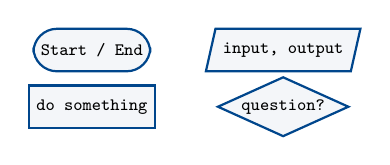
\begin{tikzpicture}[scale=0.9, every node/.style={transform shape}]
      \node[term] (a) at (0,0) {Start / End};
      \node[io]   (b) at (2.7,0) {input, output};
      \node[proc] (c) at (0,-0.8) {do something};
      \node[dec]  (d) at (2.7,-0.8) {question?};
    \end{tikzpicture}
    \vspace{0.2em}
    \begin{discussionbox}{Draw it, then answer}
      \small
      \textbf{1.} Draw the whole flowchart. Every \code{for} unpacks into three shapes ---
      which?\\[0.25em]
      \textbf{2.} The \code{do-while} and the \code{for}: where is each one's diamond,
      compared with its body?\\[0.25em]
      \textbf{3.} Where does the \code{break} arrow go?\\[0.25em]
      \textbf{4.} How many arrows point \emph{into} the diamond \code{j * j <= i}? Into
      \code{i <= n}?
    \end{discussionbox}
  \end{columns}
\end{frame}

\begin{frame}{Draw it: one answer}
  \begin{columns}[T,onlytextwidth]
    \column{0.74\textwidth}
    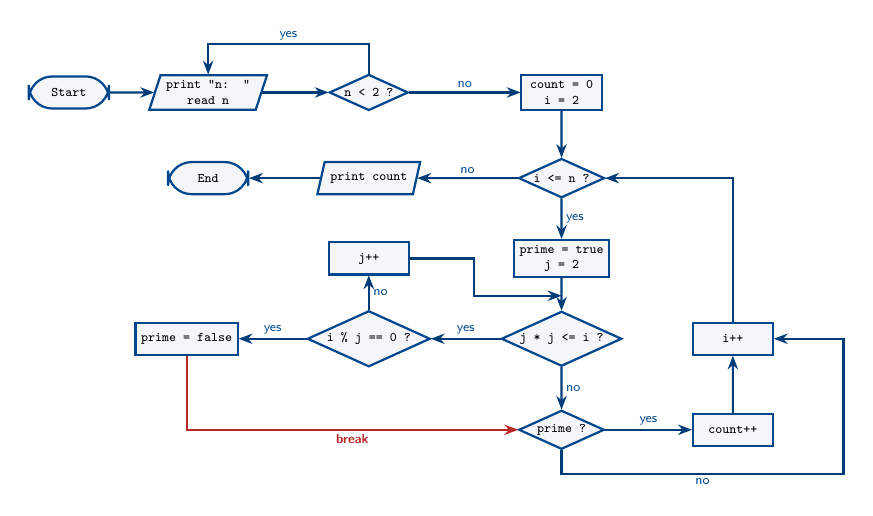
\begin{tikzpicture}[scale=0.68, every node/.style={transform shape}]
      % the do-while
      \node[term] (start) at (0,0) {Start};
      \node[io]   (in)    at (2.6,0) {print "n: "\\read n};
      \node[dec]  (d1)    at (5.6,0) {n < 2 ?};
      \node[proc] (init)  at (9.2,0) {count = 0\\i = 2};
      % the outer loop test, and the way out
      \node[dec]  (d2)    at (9.2,-1.6) {i <= n ?};
      \node[io]   (out)   at (5.6,-1.6) {print count};
      \node[term] (stop)  at (2.6,-1.6) {End};
      % the outer body
      \node[proc] (p2)    at (9.2,-3.1) {prime = true\\j = 2};
      \node[dec]  (d3)    at (9.2,-4.6) {j * j <= i ?};
      \node[dec]  (d4)    at (5.6,-4.6) {i \% j == 0 ?};
      \node[proc] (jinc)  at (5.6,-3.1) {j++};
      \node[proc] (pf)    at (2.2,-4.6) {prime = false};
      \node[dec]  (d5)    at (9.2,-6.3) {prime ?};
      \node[proc] (cnt)   at (12.4,-6.3) {count++};
      \node[proc] (iinc)  at (12.4,-4.6) {i++};

      \draw[arr] (start) -- (in);
      \draw[arr] (in) -- (d1);
      \draw[arr] (d1.north) -- ++(0,0.55) -| node[lbl, pos=0.25, above] {yes} (in.north);
      \draw[arr] (d1) -- node[lbl, above] {no} (init);
      \draw[arr] (init) -- (d2);
      \draw[arr] (d2) -- node[lbl, above] {no} (out);
      \draw[arr] (out) -- (stop);
      \draw[arr] (d2) -- node[lbl, right] {yes} (p2);
      \draw[arr] (p2) -- (d3);
      \draw[arr] (d3) -- node[lbl, above] {yes} (d4);
      \draw[arr] (d4) -- node[lbl, right] {no} (jinc);
      \draw[arr] (jinc.east) -- ++(1.2,0) |- ([yshift=0.28cm]d3.north) ;
      \draw[arr] (d4) -- node[lbl, above] {yes} (pf);
      \draw[arr, draw=badred] (pf.south) |- node[lbl, pos=0.75, below, text=badred] {\textbf{break}} (d5.west);
      \draw[arr] (d3) -- node[lbl, right] {no} (d5);
      \draw[arr] (d5) -- node[lbl, above] {yes} (cnt);
      \draw[arr] (cnt) -- (iinc);
      \draw[arr] (d5.south) -- ++(0,-0.45) -| node[lbl, pos=0.25, below] {no} ([xshift=1.3cm]iinc.east) -- (iinc.east);
      \draw[arr] (iinc.north) |- (d2.east);
    \end{tikzpicture}
    \column{0.24\textwidth}
    \footnotesize\raggedright
    \textbf{1.} Start value, diamond, update --- \code{i = 2}, \code{i <= n ?},
    \code{i++}\\[0.3em]
    \textbf{2.} \code{do-while}: diamond \textbf{after} the body. \code{for}: diamond
    \textbf{before} it\\[0.3em]
    \textbf{3.} Out of the inner loop only --- to \code{prime ?}, skipping \code{j++}\\[0.3em]
    \textbf{4.} Two each: one from the start value, one from the update. Every loop has
    an arrow going \textbf{back}
  \end{columns}
\end{frame}

% ======================================================================
\section{Team round 2: spot the errors}
% ======================================================================

\begin{frame}[fragile]{Spot the errors 1: primes, in Java \timing{Teams}{4 min}}
  \begin{columns}[T,onlytextwidth]
    \column{0.56\textwidth}
    \badlabel{Should print every prime below n, then how many.}
\begin{lstlisting}[style=bad, language=Java, numbers=left, numberstyle=\tiny\color{codegray}, numbersep=0.9em]
int n = sc.nextInt();

next:
for (int i = 1; i <= n; i++) {
    int count = 0;
    for (int j = 2; j < i; i++) {
        if (i % j == 0) break;
    }
    count++;
    System.out.println(i + " is prime.");
}
System.out.println(count + " primes below " + n);
\end{lstlisting}
    \column{0.40\textwidth}
    \begin{discussionbox}{Three tasks}
      \small
      \textbf{1.} There are \textbf{five} bugs. Find them all, with line numbers.\\[0.3em]
      \textbf{2.} Only one of the five stops it compiling. Which?\\[0.3em]
      \textbf{3.} Fix \emph{only} that one. Now what does it print for \code{n = 10}?
      (Trace it. It is not what you expect.)
    \end{discussionbox}
    \vspace{0.3em}
    {\small For \code{n = 10} it should print 2, 3, 5, 7 and \code{4 primes below 10}.}
  \end{columns}
\end{frame}

\begin{frame}[fragile]{Spot the errors 1: answers}
  \begin{columns}[T,onlytextwidth]
    \column{0.52\textwidth}
    \begin{contextbox}{The five bugs}
      \small\raggedright
      \textbf{L4} \code{i = 1}: 1 is not prime --- and the inner loop never runs for it\\[0.1em]
      \textbf{L4} \code{i <= n}: ``below \code{n}'' means \code{i < n}\\[0.1em]
      \textbf{L5} \code{count} inside the loop: reset to 0 every pass, and gone after the
      loop --- line 12 \textbf{does not compile}\\[0.1em]
      \textbf{L6} \code{i++} in the inner header: it must change \textbf{its own}
      variable, \code{j}\\[0.1em]
      \textbf{L7} \code{break} ends only the inner loop, so lines 9--10 still run. It needs
      \code{continue next} --- the unused label was a clue
    \end{contextbox}
    \column{0.44\textwidth}
    \neutrallabel{3. With only the compile error fixed, \code{n = 10}:}
\begin{lstlisting}[style=bad]
1 is prime.
2 is prime.
4 is prime.
6 is prime.
8 is prime.
10 is prime.
6 primes below 10
\end{lstlisting}
    {\small At \code{i = 3} the inner loop bumps \code{i} to 4, then \code{4 \% 2 == 0}
    breaks --- and the \emph{even} number is announced. The bugs work together to produce
    almost exactly the wrong list.}
  \end{columns}
  \keyline{The compiler found one bug in five. The other four needed a trace.}
\end{frame}

\begin{frame}[fragile]{Spot the errors 2: odd numbers, in Python \timing{Teams}{3 min}}
  \begin{columns}[T,onlytextwidth]
    \column{0.54\textwidth}
    \badlabel{Should sum the odd numbers from 1 to n.}
\begin{lstlisting}[style=bad, language=Py, numbers=left, numberstyle=\tiny\color{codegray}, numbersep=0.9em]
n = input("n: ")
total = 0
i = 1
while (i <= n) {
    if i % 2 == 0:
        continue
    total += i
    i++
}
print("Sum of odd numbers up to " + n
      + " is " + total)
\end{lstlisting}
    {\small Written by someone who learnt Java first. For \code{n = 10} it should print
    \code{Sum of odd numbers up to 10 is 25}.}
    \column{0.42\textwidth}
    \begin{discussionbox}{Two tasks}
      \small
      \textbf{1.} Find all \textbf{five} errors, with line numbers.\\[0.4em]
      \textbf{2.} Python shows you \textbf{one error at a time}: fix it, run again, meet the
      next. In what \textbf{order} will you meet the five? And which one never shows an
      error message at all?
    \end{discussionbox}
  \end{columns}
\end{frame}

\begin{frame}[fragile]{Spot the errors 2: answers, in the order you meet them}
  \begin{columns}[T,onlytextwidth]
    \column{0.55\textwidth}
    \begin{contextbox}{Run, fix, run again}
      \footnotesize\raggedright
      \textbf{1.} \textbf{L4, L9} \code{\{ \}} --- \code{SyntaxError}. A Python block is a
      colon and indentation\\[0.2em]
      \textbf{2.} \textbf{L8} \code{i++} --- \code{SyntaxError}. Python has no \code{++}:
      \code{i += 1}\\[0.2em]
      \textbf{3.} \textbf{L1} no \code{int()} --- \code{TypeError} on L4: \code{'<='} not
      supported between \code{int} and \code{str}\\[0.2em]
      \textbf{4.} \textbf{L6} \code{continue} --- \badlabel{no message at all.} At
      \code{i = 2} it skips \code{i += 1}, every time. The program just hangs\\[0.2em]
      \textbf{5.} \textbf{L10} \code{"..." + n} --- \code{TypeError}: can only concatenate
      \code{str} (not \code{int}). Use commas. It was there all along, hidden behind
      number 4
    \end{contextbox}
    \column{0.41\textwidth}
    \goodlabel{Fixed}
\begin{lstlisting}[style=good, language=Py]
n = int(input("n: "))
total = 0
i = 1
while i <= n:
    if i % 2 == 1:
        total += i
    i += 1
print("Sum of odd numbers up to", n,
      "is", total)
\end{lstlisting}
    {\footnotesize Add the odd ones instead of skipping the even ones: no \code{continue},
    no trap.}
  \end{columns}
  \keyline{Syntax errors come first, run-time errors next, and the silent one last.}
\end{frame}

\begin{frame}[fragile]{Spot the errors 3: logic only \timing{Teams}{5 min}}
  \begin{columns}[T,onlytextwidth]
    \column{0.50\textwidth}
    \badlabel{It compiles. It runs. Five logic errors.}
\begin{lstlisting}[style=bad, language=Java, numbers=left, numberstyle=\tiny\color{codegray}, numbersep=0.9em]
int n = sc.nextInt();
int limit = sc.nextInt();
int total = 0;
int sum = 0;
for (int i = 1; i < n; i++) {
    for (int j = 1; j < i; j++) {
        sum += j;
        if (sum > limit) break;
    }
    System.out.println(i + ": " + sum);
    total = sum;
}
System.out.println("Total: " + total);
\end{lstlisting}
    \column{0.46\textwidth}
    {\footnotesize \textbf{Should:} for each row \code{i} from 1 to \code{n}, print
    1 + 2 + \ldots{} + \code{i}. Stop \textbf{everything} the moment a sum goes over
    \code{limit}. Then print the total of the rows printed.\par}
    \vspace{0.3em}
    {\footnotesize
    \code{5, 100} $\to$ \code{1: 1} \ldots{} \code{5: 15}, \code{Total: 35}\\
    \code{5, 8} $\to$ \code{1: 1}, \code{2: 3}, \code{3: 6}, \code{Total: 10}}
    \vspace{0.3em}
    \begin{discussionbox}{Three tasks}
      \small
      \textbf{1.} Find all five (line numbers). Fix each.\\[0.2em]
      \textbf{2.} What does it print for \code{5, 100}?\\[0.2em]
      \textbf{3.} For \code{5, 8} it ends \code{Total: 10} --- correct! Why is that no
      comfort?
    \end{discussionbox}
  \end{columns}
\end{frame}

\begin{frame}[fragile]{Spot the errors 3: answers}
  \begin{columns}[T,onlytextwidth]
    \column{0.52\textwidth}
    \begin{contextbox}{The five, and their fixes}
      \footnotesize\raggedright
      \textbf{L4} \code{sum} is never reset: declare \code{int sum = 0;} \textbf{inside}
      the outer loop, so each row starts from 0\\[0.15em]
      \textbf{L5} \code{i < n} misses the last row: \code{i <= n}\\[0.15em]
      \textbf{L6} \code{j < i} misses \code{i} itself: \code{j <= i}\\[0.15em]
      \textbf{L8} \code{break} ends only the \emph{inner} loop: the row is still printed and
      the next row starts. Label the outer loop \code{rows:} and \code{break rows;}\\[0.15em]
      \textbf{L11} \code{total = sum} keeps only the last row: \code{total += sum}
    \end{contextbox}
    \column{0.44\textwidth}
    \neutrallabel{2. The buggy version, for \code{5, 100}}
\begin{lstlisting}[style=bad]
1: 0
2: 1
3: 4
4: 10
Total: 10
\end{lstlisting}
    {\small \textbf{3.} For \code{5, 8} it prints \code{Total: 10} too --- by accident,
    after four wrong rows. One right number proves nothing: \textbf{check every line}, and
    test more than one input.}
  \end{columns}
  \keyline{Every one of these compiles. Only a trace, or a test, finds them.}
\end{frame}

% ======================================================================
\section{Team round 3: predict the output}
% ======================================================================

\begin{frame}[fragile]{Predict 1: four loops, two claims \timing{Teams}{4 min}}
  {\small The lecture: a \code{for} is a \code{while} with its parts unpacked; a \code{do-while}
  tests afterwards. Test those claims.}
  \begin{columns}[T,onlytextwidth]
    \column{0.49\textwidth}
    \neutrallabel{Pair A}
\begin{lstlisting}[language=Java]
for (int i = 0; i < 10; i++) {
    if (i % 3 == 0) continue;
    System.out.print(i + " ");
}
\end{lstlisting}
    \vspace{-0.6em}
\begin{lstlisting}[language=Java]
int i = 0;
while (i < 10) {
    if (i % 3 == 0) continue;
    System.out.print(i + " ");
    i++;
}
\end{lstlisting}
    \column{0.47\textwidth}
    \neutrallabel{Pair B} \small (\code{n} is read from the user)
\begin{lstlisting}[language=Java]
int k = 0;
while (k < n) {
    System.out.print(k + " ");
    k++;
}
\end{lstlisting}
    \vspace{-0.6em}
\begin{lstlisting}[language=Java]
int k = 0;
do {
    System.out.print(k + " ");
    k++;
} while (k < n);
\end{lstlisting}
  \end{columns}
  \vspace{-0.5em}
  \begin{discussionbox}{For each pair}
    \small Write exactly what each of the four loops prints --- pair B for \code{n = 3}, then
    \code{n = 0}. Which pair behaves the same for \textbf{every} input?
  \end{discussionbox}
\end{frame}

\begin{frame}[fragile]{Predict 1: answers}
  \begin{columns}[T,onlytextwidth]
    \column{0.50\textwidth}
    \badlabel{Pair A: not the same}
    \begin{itemize}[itemsep=0.15em]
      \small
      \item The \code{for} prints \code{1 2 4 5 7 8}
      \item The \code{while} prints \textbf{nothing, forever}. At \code{i = 0},
        \code{continue} jumps straight back to the condition --- \textbf{past} the
        \code{i++} at the bottom
      \item In a \code{for}, \code{continue} jumps to the \textbf{modification part}, so
        \code{i++} still happens
    \end{itemize}
    \goodlabel{One fix}
\begin{lstlisting}[style=good, language=Java]
int i = 0;
while (i < 10) {
    if (i % 3 == 0) { i++; continue; }
    System.out.print(i + " ");
    i++;
}
\end{lstlisting}
    \column{0.46\textwidth}
    \badlabel{Pair B: same until n $\le$ 0}
    \begin{itemize}[itemsep=0.15em]
      \small
      \item For \code{n} = 3, both print \code{0 1 2}
      \item For \code{n} = 0 (or any negative), the \code{while} prints nothing and the
        \code{do-while} prints \code{0}
      \item The difference only shows when the condition is false \textbf{the first time}
    \end{itemize}
    \vspace{0.4em}
    \begin{contextbox}{The lesson}
      \small ``Equivalent'' means for \emph{every} input. One counter-example is enough to
      break the claim --- and it is almost always a boundary: zero passes, or a
      \code{continue}.
    \end{contextbox}
  \end{columns}
\end{frame}

\begin{frame}[fragile]{Predict 2: the mystery loop \timing{Teams}{4 min}}
  \begin{columns}[T,onlytextwidth]
    \column{0.47\textwidth}
\begin{lstlisting}[language=Java]
int n = sc.nextInt();
int r = 0;
while (n > 0) {
    r = r * 10 + n % 10;
    n = n / 10;
}
System.out.println(r);
\end{lstlisting}
    \vspace{0.2em}
    {\small Trace it for \code{472} with a table:}\\[0.3em]
    {\small
    \renewcommand{\arraystretch}{1.1}
    \begin{tabular}{@{}c|c|c|c@{}}
      pass & \code{n \% 10} & \code{r} & \code{n}\\
      \hline
      start & --- & 0 & 472\\
      1 & & & \\
      \ldots & & & \\
    \end{tabular}}
    \column{0.49\textwidth}
    \begin{discussionbox}{Four tasks}
      \small
      \textbf{1.} Finish the trace. What prints?\\[0.3em]
      \textbf{2.} In one sentence: what does this loop compute?\\[0.3em]
      \textbf{3.} What prints for \code{1200}? \code{7}? \code{0}? \code{-45}? Which of
      those are wrong answers?\\[0.3em]
      \textbf{4.} Someone adds, after the loop:\\
      \code{if (r == n) System.out.println("palindrome");}\\
      What prints for \code{1221}? Why?
    \end{discussionbox}
  \end{columns}
\end{frame}

\begin{frame}[fragile]{Predict 2: answers}
  \begin{columns}[T,onlytextwidth]
    \column{0.46\textwidth}
    {\small
    \renewcommand{\arraystretch}{1.1}
    \begin{tabular}{@{}c|c|c|c@{}}
      pass & \code{n \% 10} & \code{r} & \code{n}\\
      \hline
      start & --- & 0 & 472\\
      1 & 2 & 2 & 47\\
      2 & 7 & 27 & 4\\
      3 & 4 & 274 & 0\\
    \end{tabular}}
    \vspace{0.4em}

    \textbf{1.} \code{274}\quad \textbf{2.} It \textbf{reverses the digits}: \code{\% 10}
    takes the last digit off, \code{/ 10} throws it away, \code{r * 10} makes room.
    \vspace{0.4em}

    \textbf{3.} \code{1200} $\to$ \code{21}: \code{r} is a number, and a number has no
    leading zeros. \code{7} $\to$ \code{7}. \code{0} $\to$ \code{0}. \code{-45} $\to$
    \code{0} --- \badlabel{wrong}: \code{n > 0} is false at once, zero passes.
    \column{0.50\textwidth}
    \textbf{4.} Only \code{1221} --- \textbf{no} \code{palindrome}. After the loop \code{n}
    is \textbf{0}, so it compares 1221 with 0. (For input 0 it \emph{does} say
    \code{palindrome} --- right, by accident.) Save a copy first:
\begin{lstlisting}[style=good, language=Java]
int n = sc.nextInt();
int original = n;      // missing
int r = 0;
while (n > 0) {
    r = r * 10 + n % 10;
    n = n / 10;
}
if (r == original)
    System.out.println("palindrome");
\end{lstlisting}
  \end{columns}
  \keyline{A loop that changes its variable uses it up. Keep a copy if you need it after.}
\end{frame}

% ======================================================================
\section{Team round 4: write the code}
% ======================================================================

\begin{frame}[fragile]{Code it 1: leave both loops, in Python \timing{Teams}{4 min}}
  \begin{columns}[T,onlytextwidth]
    \column{0.49\textwidth}
    \neutrallabel{Java}
\begin{lstlisting}[language=Java]
outer:
for (int i = 0; i < 3; i++) {
    for (int j = 0; j < 3; j++) {
        if (i + j == 3) break outer;
        System.out.println(i + " " + j);
    }
}
\end{lstlisting}
    \column{0.47\textwidth}
    \vspace{0.4em}
    \begin{discussionbox}{Two tasks}
      \small
      \textbf{1.} Write down the Java's full output.\\[0.3em]
      \textbf{2.} Write Python that prints \textbf{exactly} the same. Python has no
      labelled \code{break} --- and a plain \code{break} is \emph{not} the same thing.
      Check your version against your answer to 1.\\[0.5em]
      \textbf{Hard bonus.} Do task 3 \emph{without} a new variable. (Hint: a loop can
      have an \code{else}.)
    \end{discussionbox}
  \end{columns}
\end{frame}

\begin{frame}[fragile]{Code it 1: answers}
  \begin{columns}[T,onlytextwidth]
    \column{0.30\textwidth}
    \textbf{1.} Java: five lines\\
    \code{0 0}, \code{0 1}, \code{0 2}, \code{1 0}, \code{1 1}.\\
    At \code{1 2} it leaves \textbf{both} loops.
    \vspace{0.5em}

    The obvious translation --- just \code{break} --- prints \textbf{six}: the same five,
    \textbf{plus} \code{2 0}. It ends only the inner loop, so the outer one carries on with
    \code{i = 2}.
    \column{0.33\textwidth}
    \goodlabel{2. With a flag}
\begin{lstlisting}[style=good, language=Py]
found = False
for i in range(3):
    for j in range(3):
        if i + j == 3:
            found = True
            break
        print(i, j)
    if found:
        break
\end{lstlisting}
    \column{0.33\textwidth}
    \goodlabel{Bonus: loop-else}
\begin{lstlisting}[style=good, language=Py]
for i in range(3):
    for j in range(3):
        if i + j == 3:
            break
        print(i, j)
    else:
        continue
    break
\end{lstlisting}
    {\footnotesize Inner loop finished normally: the \code{else} runs, \code{continue}
    to the next \code{i}. Inner loop broken out of: the \code{else} is skipped and the
    outer \code{break} runs.}
  \end{columns}
  \keyline{Clever --- but most people will need a minute to read it. The flag is clearer.}
\end{frame}

\begin{frame}[fragile]{Code it 2: Floyd's triangle, with a limit \timing{Teams}{6 min}}
  \begin{columns}[T,onlytextwidth]
    \column{0.45\textwidth}
    Read \code{rows} and \code{limit}. Print Floyd's triangle --- row 1 has one number,
    row 2 has two, and the numbers keep counting up. \textbf{Stop everything} the moment the
    next number would be over \code{limit}.
    \vspace{0.4em}

    \begin{itemize}[itemsep=0.2em]
      \small
      \item \textbf{One team} codes it in \textbf{Java} (\code{Floyd.java}), \textbf{one
        team} in \textbf{Python} (\code{floyd.py}), on the projector
      \item Every other team writes \emph{both} on paper, and shouts fixes
      \item Python has no labelled \code{break}. Remember \emph{Code it 1}
    \end{itemize}
    \column{0.51\textwidth}
    \begin{discussionbox}{Run it with all of these}
      \footnotesize
      \begin{tabular}{@{}p{0.22\linewidth}@{}p{0.76\linewidth}@{}}
        \textbf{input} & \textbf{should print}\\[0.15em]
        \code{5, 12}  & \code{1} / \code{2 3} / \code{4 5 6} / \code{7 8 9 10} /
          \code{11 12}\\[0.2em]
        \code{4, 100} & four full rows\\[0.2em]
        \code{5, 10}  & four rows, then nothing\\[0.2em]
        \code{8, 12}  & as \code{5, 12} --- \textbf{no blank lines}\\[0.2em]
        \code{3, 0}   & nothing at all\\
      \end{tabular}
    \end{discussionbox}
  \end{columns}
\end{frame}

\begin{frame}[fragile]{Code it 2: one answer in each language}
  \begin{columns}[T,onlytextwidth]
    \column{0.49\textwidth}
    \goodlabel{Java}
\begin{lstlisting}[style=good, language=Java]
int k = 1;
done:
for (int r = 1; r <= rows; r++) {
    for (int c = 1; c <= r; c++) {
        if (k > limit) break done;
        System.out.print(k + " ");
        k++;
    }
    System.out.println();
}
\end{lstlisting}
    \column{0.47\textwidth}
    \goodlabel{Python}
\begin{lstlisting}[style=good, language=Py]
k = 1
done = False
for r in range(rows):
    for c in range(r + 1):
        if k > limit:
            done = True
            break
        print(k, end=" ")
        k += 1
    if done:
        break
    print()
\end{lstlisting}
  \end{columns}
  \keyline{Same idea, two toolkits: a label in Java, a flag in Python.}
\end{frame}

\begin{frame}[fragile]{Code it 2: three ways to get it wrong}
  \begin{columns}[T,onlytextwidth]
    \column{0.31\textwidth}
    \badlabel{Plain \code{break}}
    \vspace{0.2em}

    {\small Leaves only the current row. For \code{rows 8}, \code{limit 12}, rows 6, 7 and 8
    each start, break at once, and print \textbf{three blank lines}. The
    \code{5, 12} test cannot see this bug.}
    \column{0.31\textwidth}
    \badlabel{\code{k = 1} inside the outer loop}
\begin{lstlisting}[style=bad]
1
1 2
1 2 3
1 2 3 4
\end{lstlisting}
    {\small Every row restarts. A counter that must \emph{survive} the rows lives outside
    both loops.}
    \column{0.31\textwidth}
    \badlabel{\code{range(r)} in Python}
    \vspace{0.2em}

    {\small \code{r} starts at 0, so row 1 gets \code{range(0)} --- \textbf{no numbers}.
    The first line is blank and every row is one short. Java counted \code{r} from 1;
    Python's \code{range} counts from 0.}
  \end{columns}
  \keyline{The first test alone misses the plain break. That is why there were five.}
\end{frame}

% ======================================================================
\section{Wrapping up}
% ======================================================================

\begin{frame}{You should now be able to\ldots}
  \begin{columns}[T,onlytextwidth]
    \column{0.48\textwidth}
    \neutrallabel{Week 3}
    \begin{itemize}[itemsep=0.2em]
      \small
      \item[\yes] say, for any loop, \textbf{what makes it stop} --- or that nothing does
      \item[\yes] count the passes of a loop, including a nested one whose inner bound uses
        the outer variable
      \item[\yes] tell a \code{while} from a \code{do-while} on the input that runs
        \textbf{zero} times
      \item[\yes] unpack a \code{for} into a \code{while} --- and spot the \code{continue}
        that breaks the unpacking
    \end{itemize}
    \column{0.48\textwidth}
    \neutrallabel{\phantom{Week 3}}
    \begin{itemize}[itemsep=0.2em]
      \small
      \item[\yes] predict which loop a \code{break} or \code{continue} affects, with and
        without a label
      \item[\yes] leave nested loops in Python with a \textbf{flag}
      \item[\yes] explain when a loop-\code{else} runs, and when it lies
      \item[\yes] trace a loop in a table, and keep a copy of what it uses up
    \end{itemize}
    \vspace{0.3em}
    \begin{contextbox}{If any box is unticked}
      \small Sections 05--07, quiz questions 9--15 and exercises 4--5:\\
      \srclink{https://lexuanbach.github.io/41039/weeks/week-2-3.html}{lexuanbach.github.io/41039}
    \end{contextbox}
  \end{columns}
\end{frame}

\end{document}
